\documentclass[17pt,letterpaper]{extarticle}
\usepackage{pdfpages}
\usepackage[utf8]{inputenc}
\usepackage{tocloft}
\usepackage{graphicx}
\usepackage{float}
\usepackage{tikz}
\usepackage{epstopdf}

\newcommand*\circled[1]{\tikz[baseline=(char.base)]{
            \node[shape=circle,draw,inner sep=2pt] (char) {#1};}}

\setlength{\footskip}{100pt}
\renewcommand{\cftsecleader}{\cftdotfill{\cftdotsep}}
\renewcommand{\contentsname}{Table of contents}
\setlength{\parindent}{0ex}

\makeatletter

\def\clearleftpage{\clearpage\ifodd\c@page\else
\hbox{}\newpage\if@twocolumn\hbox{}\newpage\fi\fi}

\makeatother

\title{12 Songs for Toy Xylophones \& Metallophones}
\date{Guilhem Vellut}
\author{Vol. 1 - French Children's Songs}

\begin{document}
\includepdfset{pagecommand=\thispagestyle{plain}}
\setcounter{secnumdepth}{-1}
\setcounter{page}{1}

\maketitle

\clearpage
\vspace*{\fill}

{\tiny 1st English edition - December 2018 \\ Typeset with LilyPond and \LaTeX \\
Cover logo by Freepik of FlatIcon.com\\
\newline
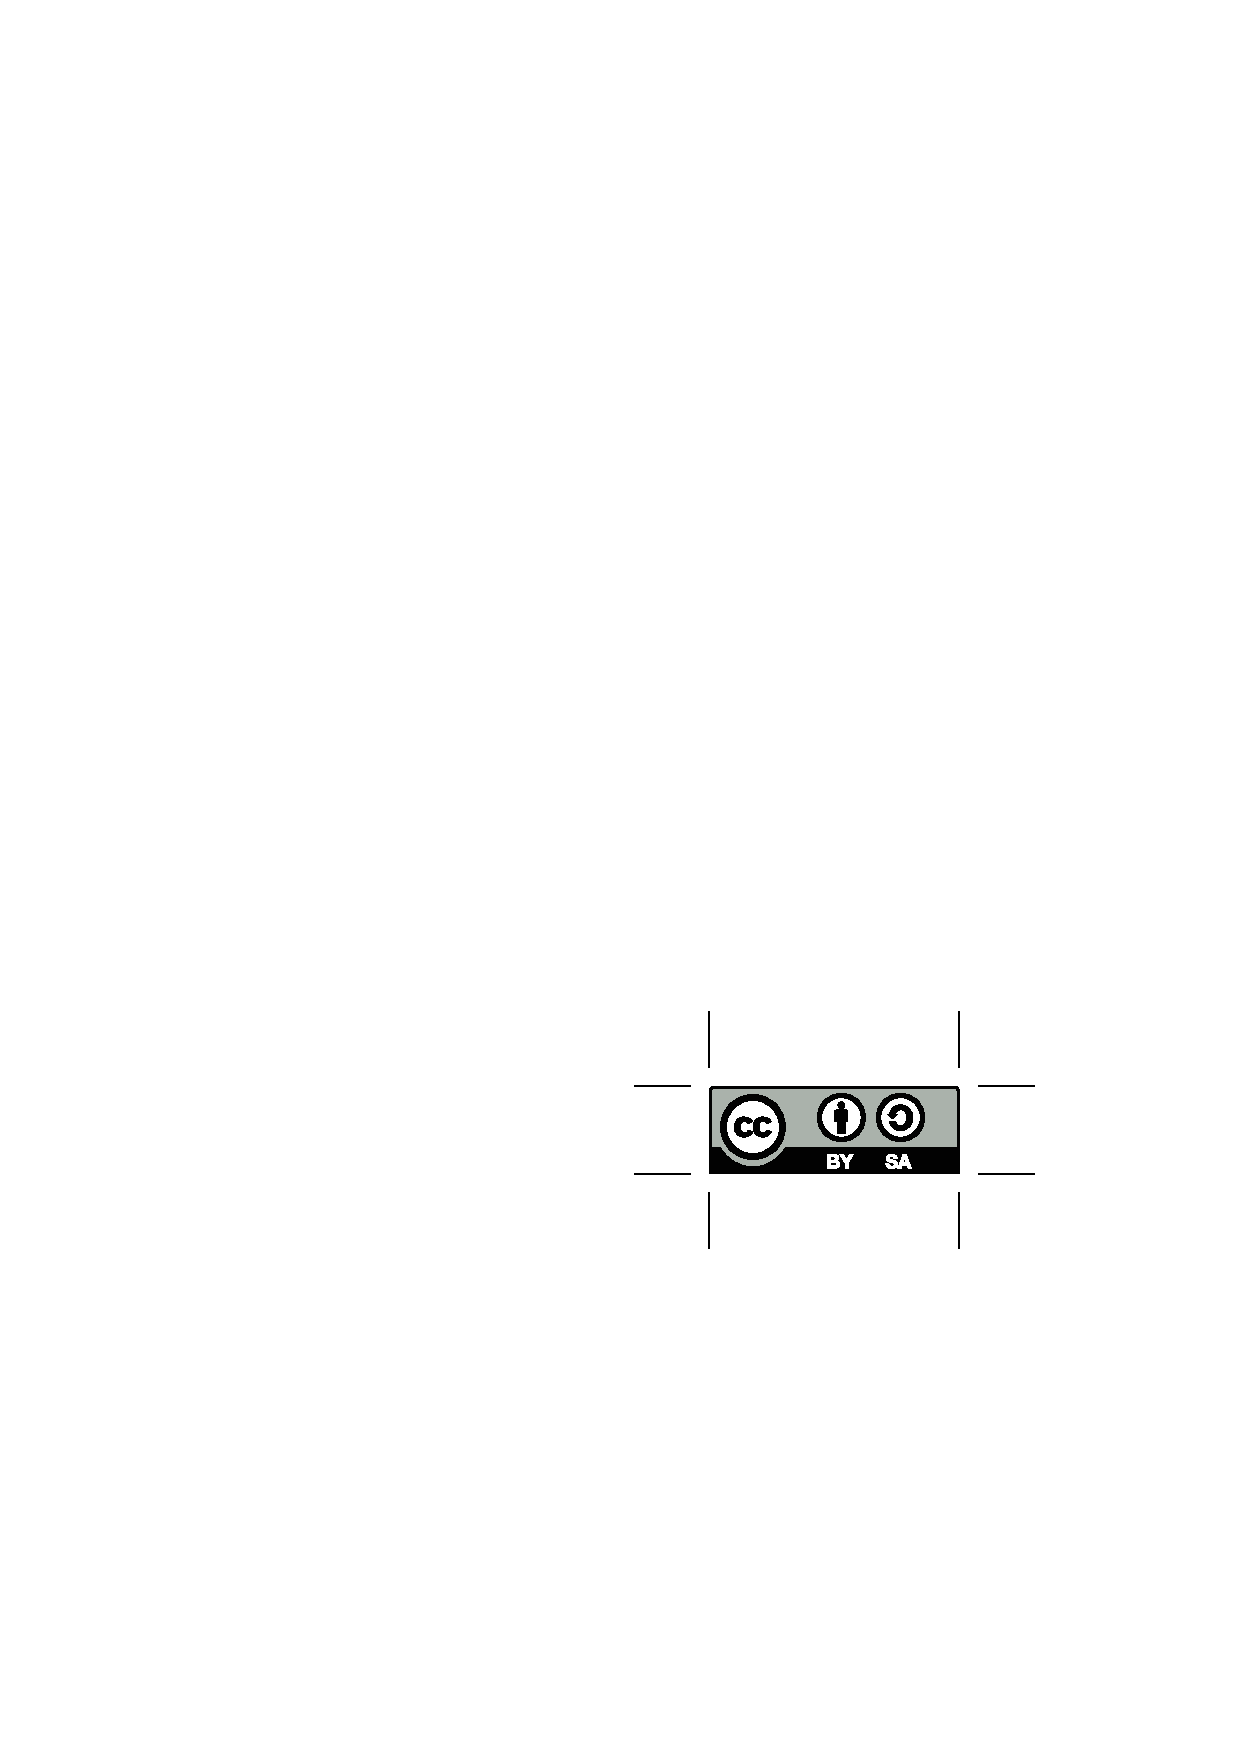
\includegraphics{by-sa} \\
\newline
Scores CC-BY-SA by Guilhem Vellut\\
Some scores have been adapted from Jean-Michel Thiémonge / Piano GNU (CC-BY)\\
Some scores have been adapted from the Wikisource Partitions project (CC-BY-SA)\\
Go to goo.gl/oMiAjK for details \par}

\clearpage

\tableofcontents

\clearleftpage

\section{Introduction \& Note colors}

This book contains sheet music of traditional French children's songs, adapted for 8-note xylopohones and metallophones (1 octave). They should be suitable for most of those instruments marketed to children, for example the Animambo Metallophone or Fisher-Price Xylophone. \\

For all the songs, I have added under each note an indication of which xylophone bar to play, so that even young children, who may not know yet how to read the standard musical notation, can follow along.\\

However, this book is printed in black \& white and the colors of the bars can be different depending on the brand of instrument. Therefore, you will have to color the hints yourself according to the color scheme of your xylophone.\\

To help you, look at the picture of a toy xylophone on the next page.\\

The bars are marked from \circled{1} to \circled{8}:
\begin{itemize}
  \item \circled{1} for the biggest bar (low C)  
  \item \circled{8} for the smallest bar (high C)
  \item Between the two C's, the bars get smaller: D \circled{2}, E \circled{3}, F  \circled{4}, G \circled{5}, A \circled{6}, B \circled{7}
\end{itemize}

\begin{figure}[h]
\centering
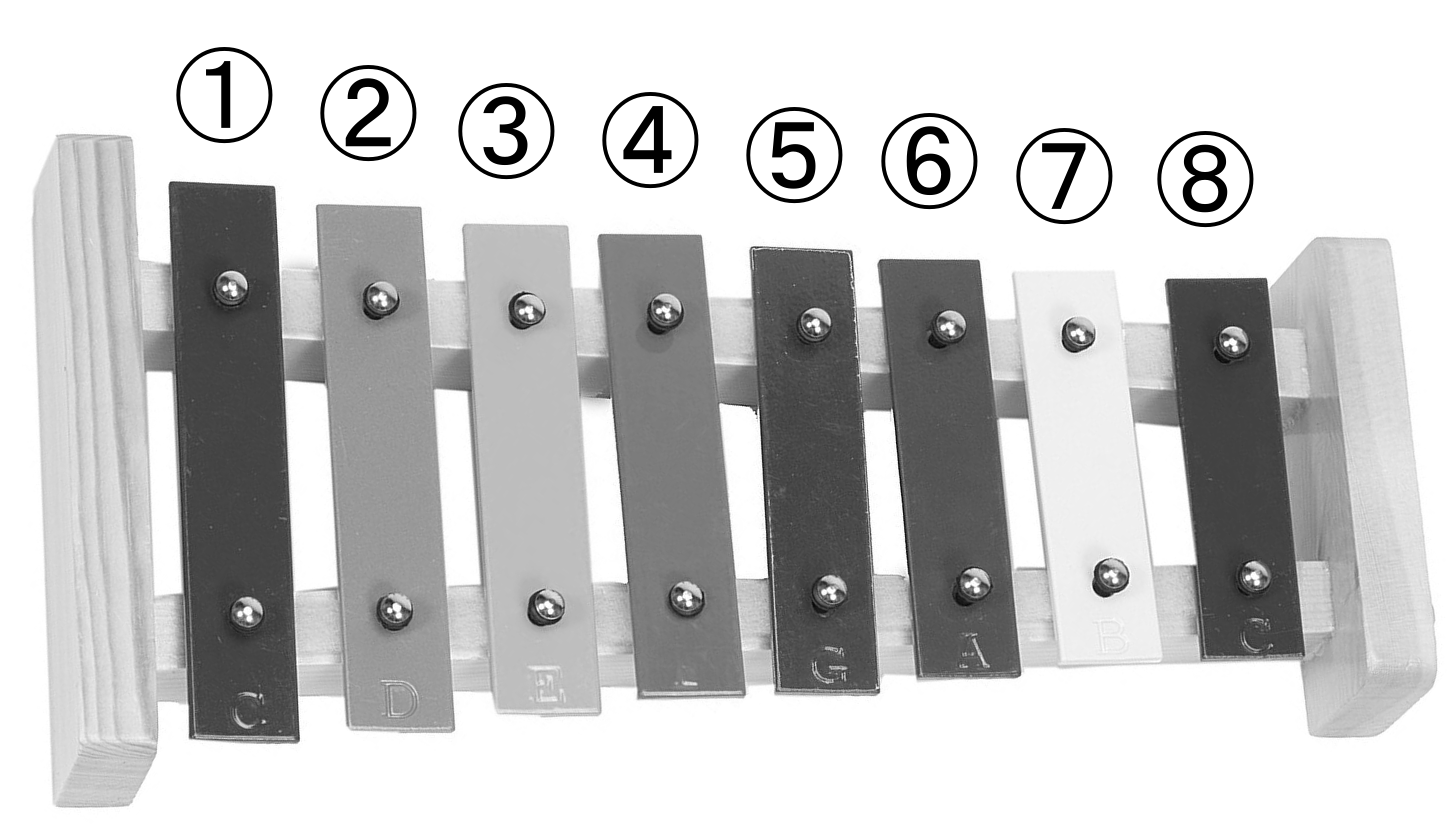
\includegraphics{xylophone_bw.png}
\end{figure}

At the beginning of all the scores in this book, you will find a list of the bars that are used in the songs, from \circled{1} to \circled{8}, like on the picture. Most songs do not use all the notes though.\\

To prepare a score for playing, you can first start by coloring those circles at the top, using the actual colors of the bars on your xylophone. Then, you can simply copy the colors for all the notes in the song. After this is done, you can finally play!\\ 

\clearleftpage

\addcontentsline{toc}{section}{Au clair de la Lune}
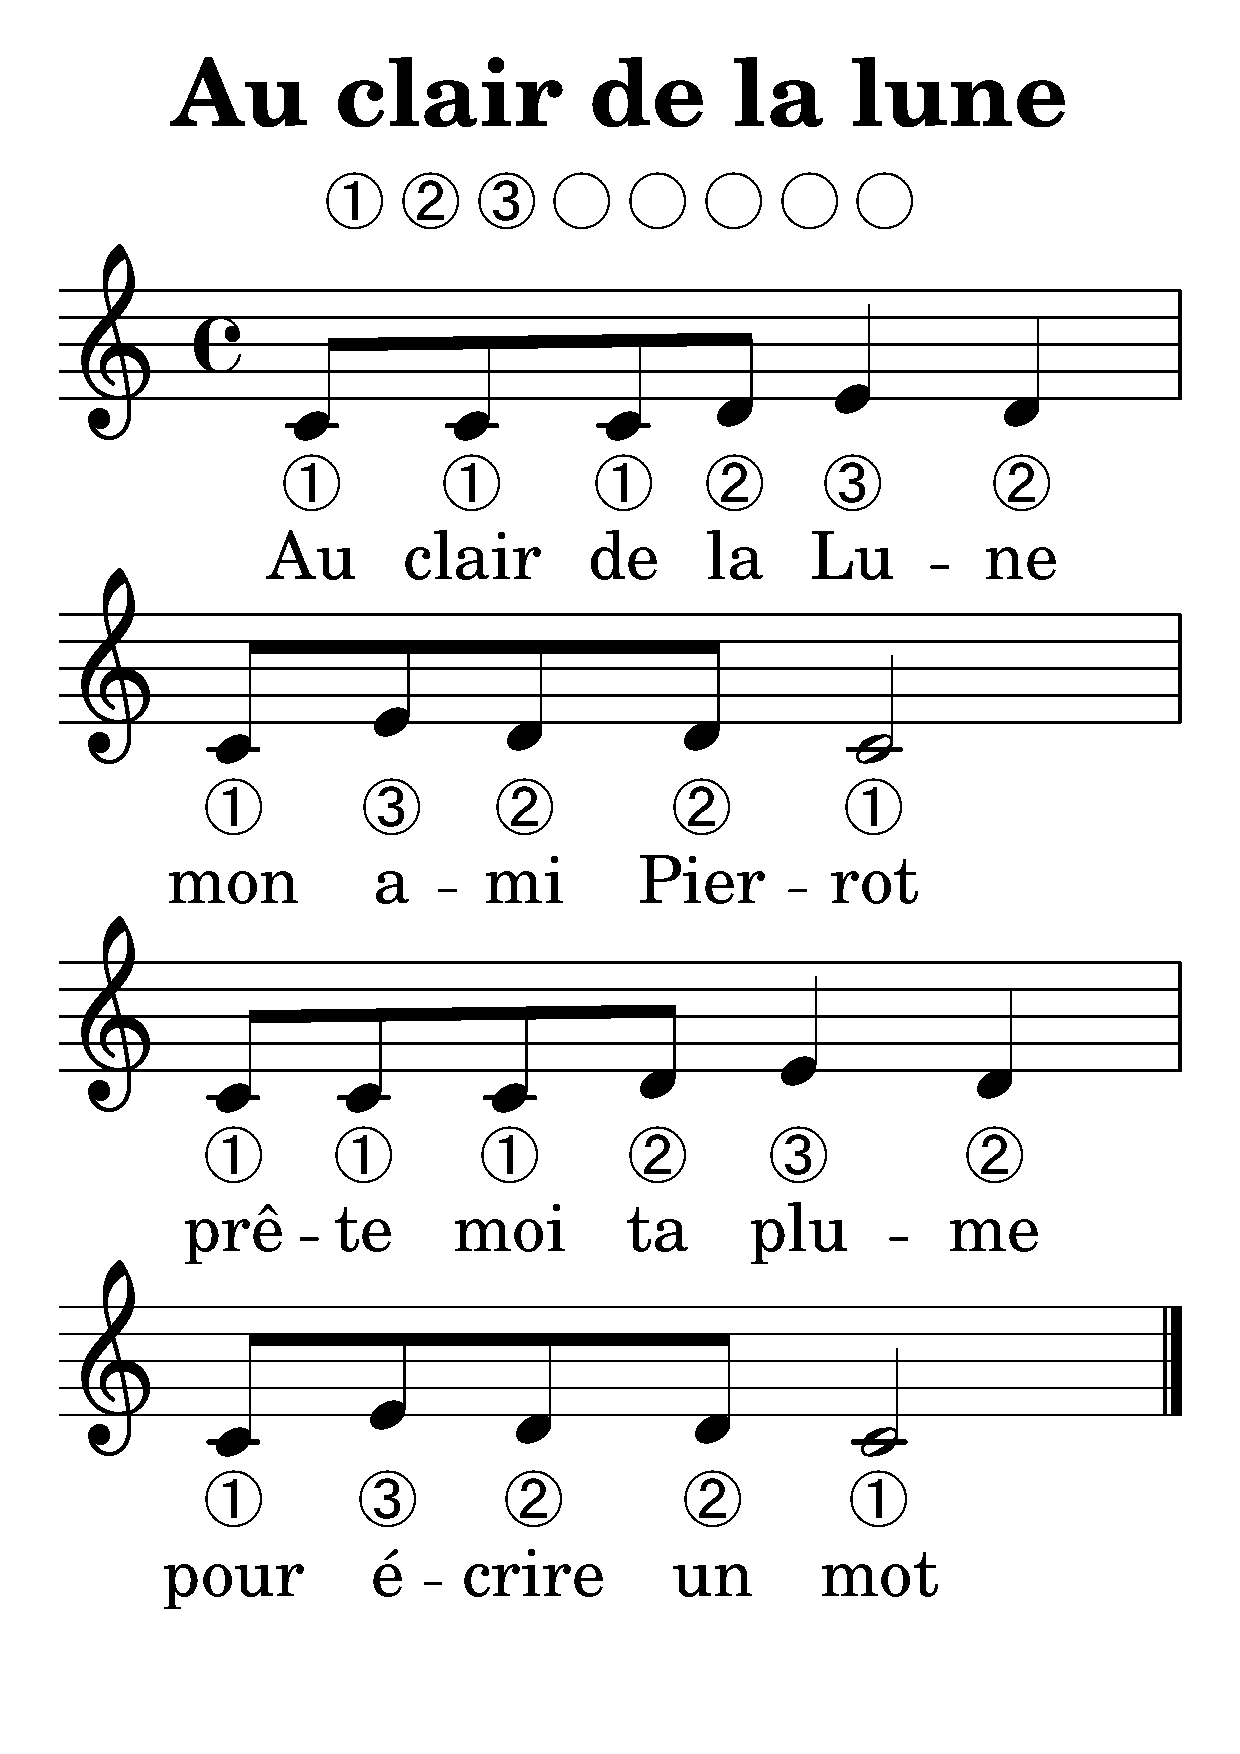
\includepdf[pages=1-,pagecommand={\null\clearpage}]{au_clair_de_la_lune.pdf}

\clearleftpage

\addcontentsline{toc}{section}{L'alphabet}
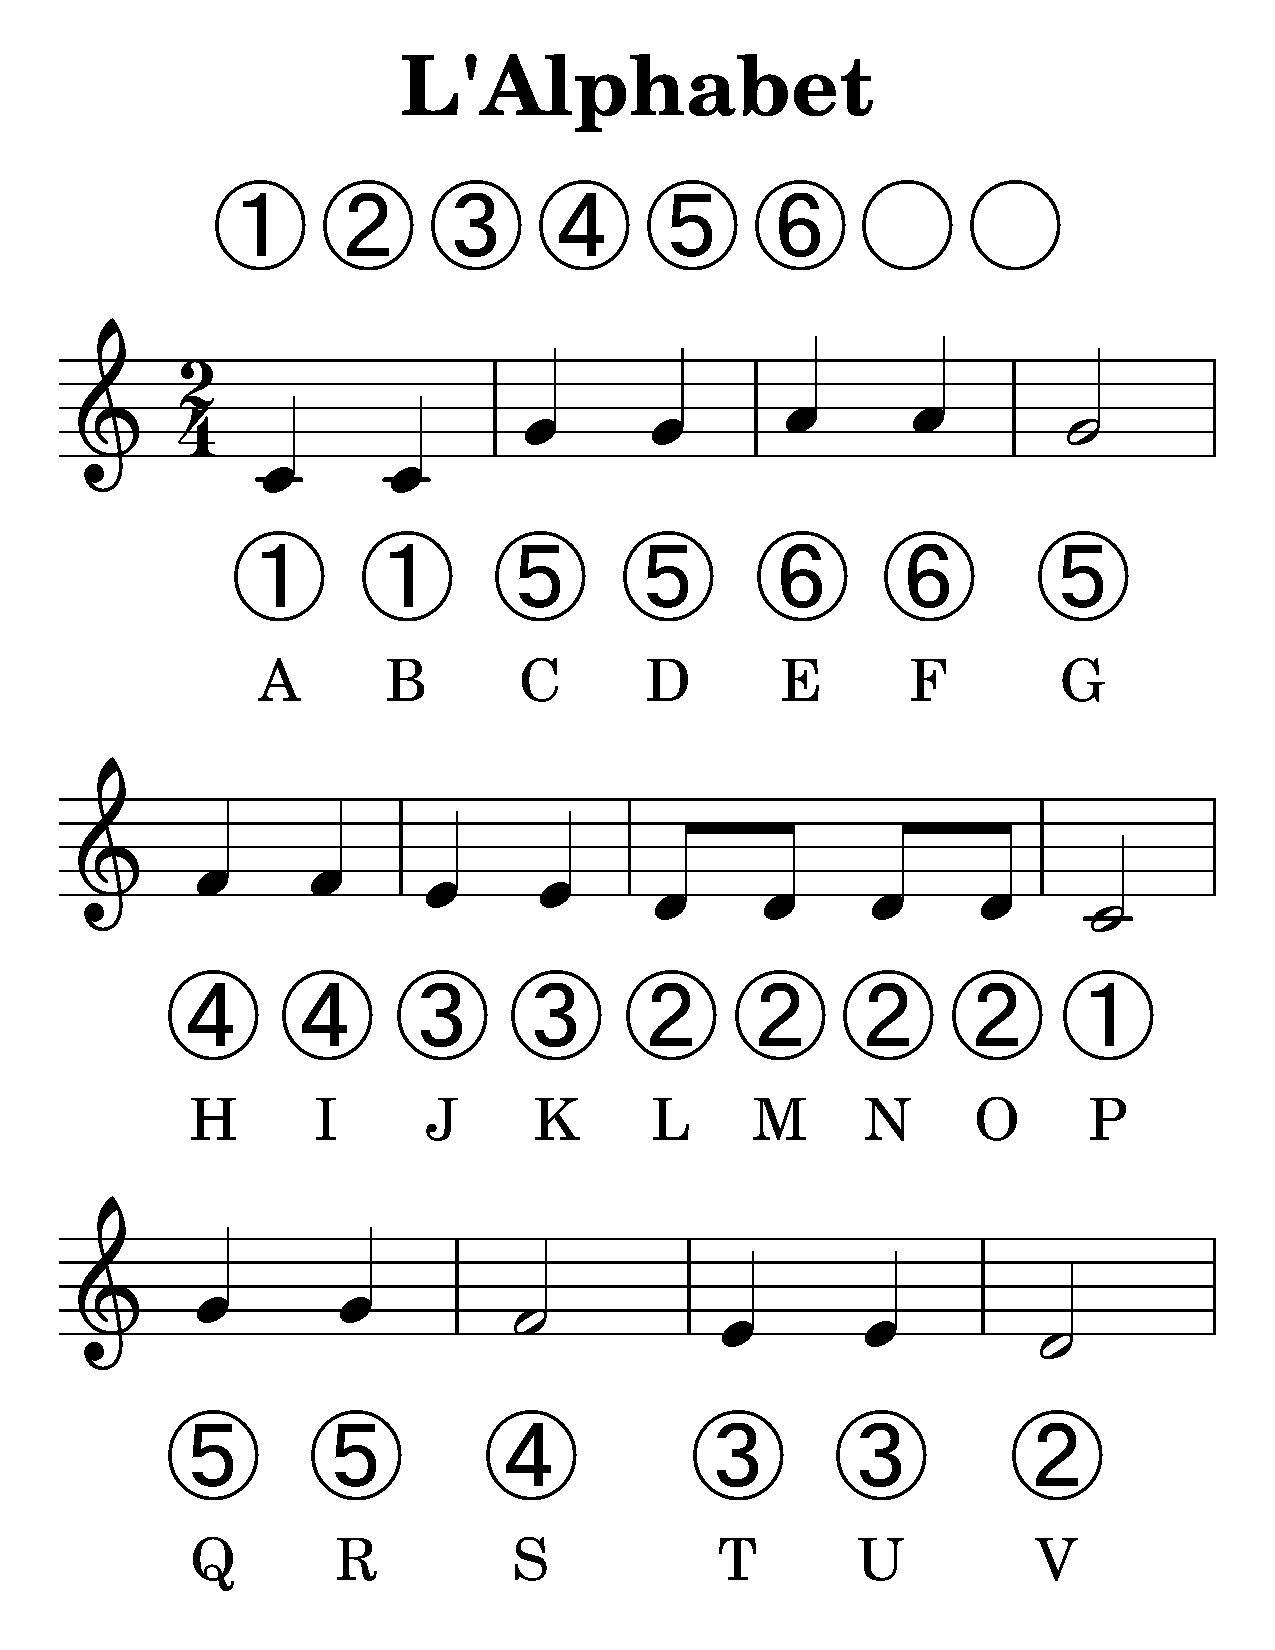
\includepdf[pages=1-,pagecommand={\null\clearpage}]{alphabet_fr.pdf}

\clearleftpage

\addcontentsline{toc}{section}{Pirouette Cacahuète}
\includepdf[pages=1-,pagecommand={\null\clearpage}]{pirouette.pdf}

\clearleftpage

\addcontentsline{toc}{section}{Dansons la capucine}
\includepdf[pages=1-,pagecommand={\null\clearpage}]{dansons_la_capucine.pdf}

\clearleftpage

\addcontentsline{toc}{section}{Il court, il court, le furet}
\includepdf[pages=1-,pagecommand={\null\clearpage}]{furet.pdf}

\clearleftpage

\addcontentsline{toc}{section}{Promenons-nous dans les bois}
\includepdf[pages=1-,pagecommand={\null\clearpage}]{promenons_nous.pdf}

\clearleftpage

\addcontentsline{toc}{section}{Vive le vent (Jingle Bells)}
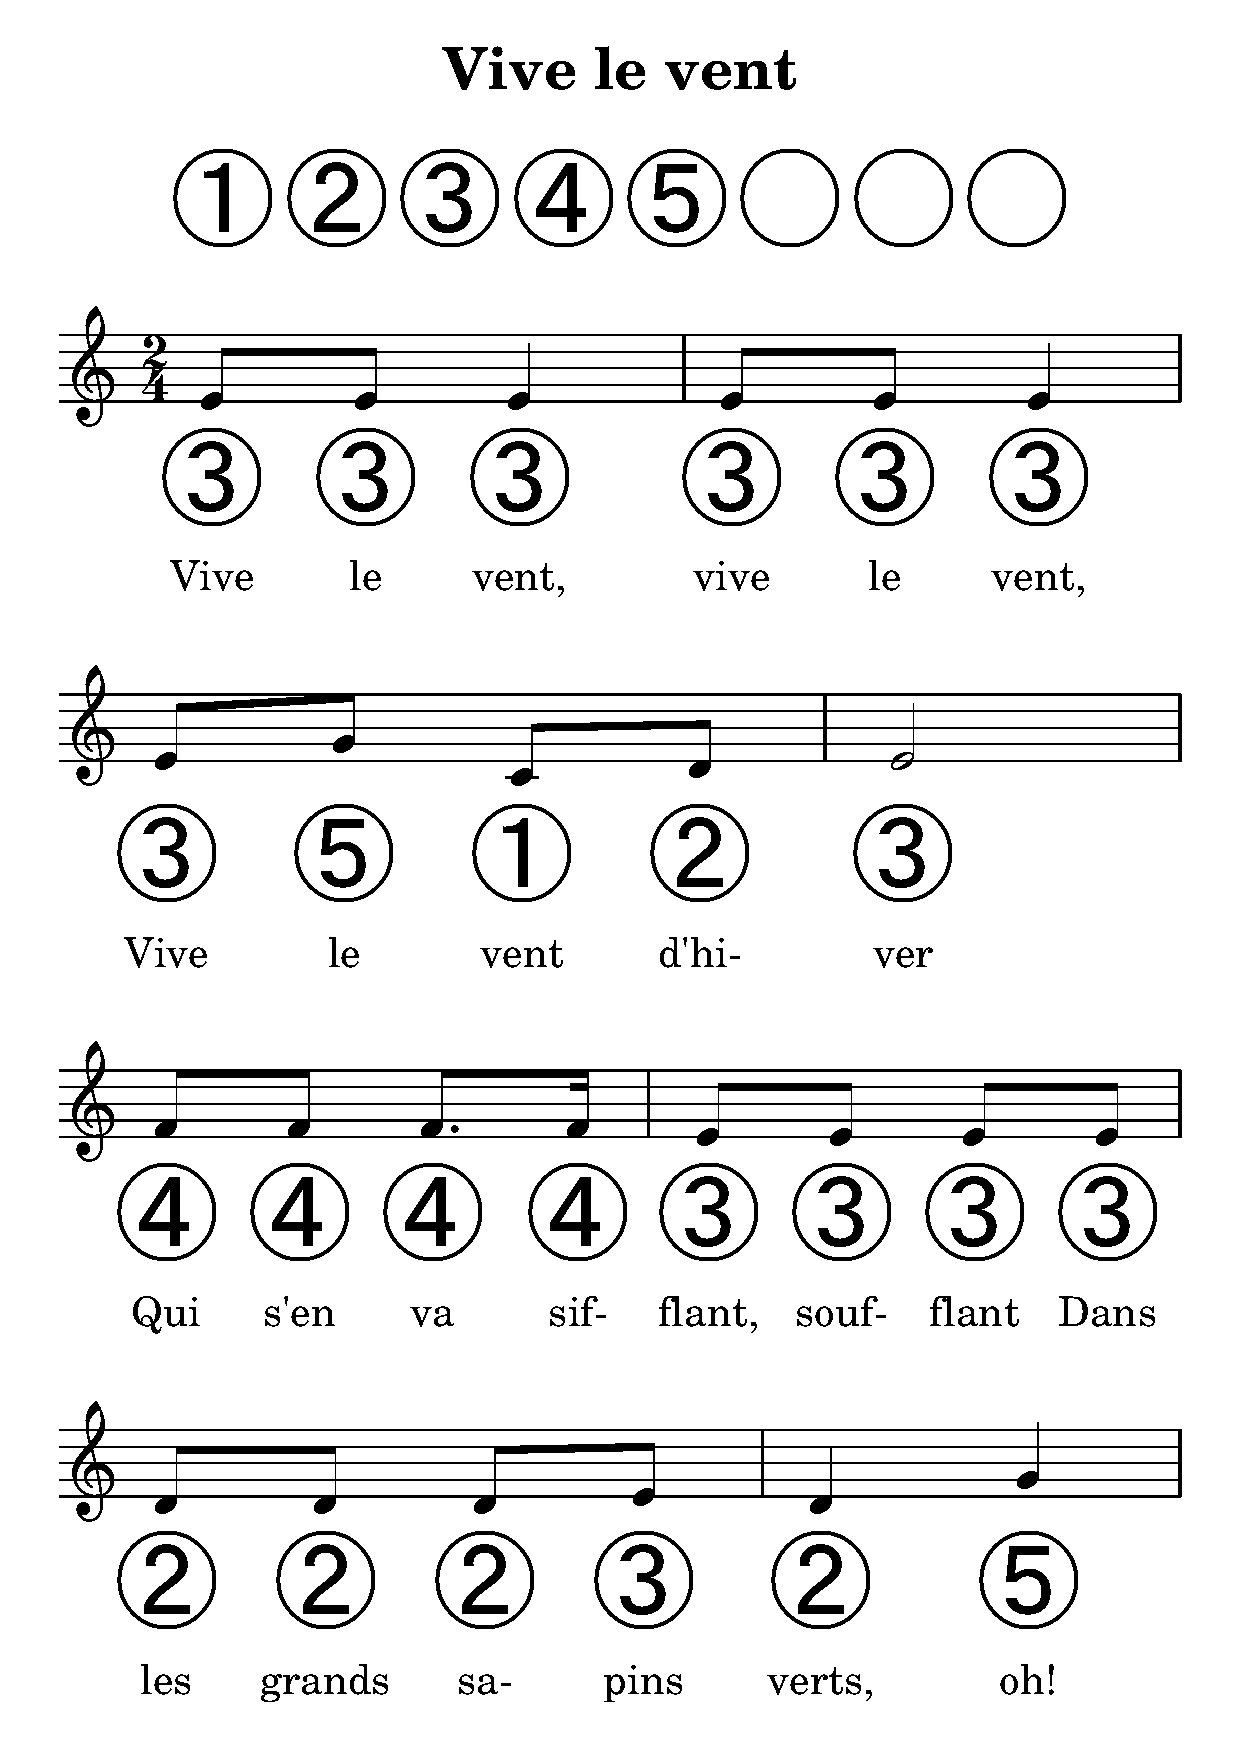
\includepdf[pages=1-,pagecommand={\null\clearpage}]{vive_le_vent.pdf}

\clearleftpage

\addcontentsline{toc}{section}{Frère Jacques}
\includepdf[pages=1-,pagecommand={\null\clearpage}]{frere_jacques.pdf}

\clearleftpage

\addcontentsline{toc}{section}{À la claire fontaine}
\includepdf[pages=1-,pagecommand={\null\clearpage}]{a_la_claire_fontaine.pdf}

\clearleftpage

\addcontentsline{toc}{section}{Le roi Dagobert}
\includepdf[pages=1-,pagecommand={\null\clearpage}]{dagobert.pdf}

\clearleftpage

\addcontentsline{toc}{section}{À la pêche aux moules}
\includepdf[pages=1-,pagecommand={\null\clearpage}]{a_la_peche_aux_moules.pdf}

\clearleftpage

\addcontentsline{toc}{section}{Bonjour, belle Rosinne}
\includepdf[pages=1-,pagecommand={\null\clearpage}]{rosinne.pdf}


\end{document}
